\chapter{Feature Extraction}
\label{ch:feature-extraction}

As an acoustic wave propagated through space over time, the speech signal is not
appropriate to be evaluated by the speaker verification system. In order to deliver
decent outcomes, a good parametric representation must be provided to the system.
This task is performed by the feature extraction process, which transforms a speech
signal into a sequence of characterized measurements, i.e. features. As stated in
\cite{davis.mermelstein.1980}, ``the usual objectives in selecting a representation
are to compress the speech data by eliminating information not pertinent to the
phonetic analysis of the data, and to enhance those aspects of the signal that
contribute significantly to the detection of phonetic differences". According to
\cite{wolf.1972} the ideal features should:

\begin{itemize}\itemsep0pt
    \item occur naturally and frequently in normal speech;
    \item be easily measurable;
    \item vary highly among speakers and be very consistent for each speaker;
    \item not change over time nor be affected by the speaker's health;
    \item be robust to reasonable background noise and to transmission
    characteristics;
    \item be difficult to be artificially produced;
    \item not be easily modifiable by the speaker.
\end{itemize}

Features may be categorized based on vocal tract or behavioral aspects, divided
in (1) short-time spectral, (2) spectro-temporal, (3) prosodic and (4) high
level \cite{pinheiro.2013}. Short-time spectral features are usually calculated
using millisecond length windows and describe the voice spectral envelope, composed
of supralaryngeal properties of the vocal tract, e.g. timbre. Prosodic and
spectro-temporal occur over time, e.g. rhythm and intonation, and high level features
occur during the conversation, e.g. accents.

The parametric representations evaluated in \cite{davis.mermelstein.1980} may
be divided into those based on the Fourier spectrum, Mel-Frequency Cepstrum
Coefficients (MFCC) and Linear Frequency Cepstrum Coefficients (LFCC), and those
based on the Linear Prediction Spectrum, Linear Prediction Coefficients (LPC),
Reflection Coefficients (RC) and Linear Prediction Cepstrum Coefficients (LPCC).
The better evaluated representation was the MFCC, with minimum and maximum accuracy
of 90.2\% and 99.4\% respectively, leading to its choice as the parametric
representation in this work.

\newpage


\section{Mel-Frequency Cepstral Coefficient}

MFCC is a highly used parametric representation in the area of voice processing,
due to its similarity with the mode the human ear operates. Despite the fact the
ear is divided in three sections, i.e. outer, middle and inner ears, only the last
is mimicked. The mechanical pressure waves produced by the triad hammer-anvil-stirrup
are received by the cochlea (\figureref{cochlea}), a spiral-shaped cavity with a
set of inner hair cells attached to a membrane (the basilar membrane) and filled
with a liquid. This structure converts motion to neural activity through a non-uniform
spectral analysis \cite{rabiner.schafer.2007} and passes it to the pattern
recognition in the brain.

\begin{figure}[ht]
    \centering
    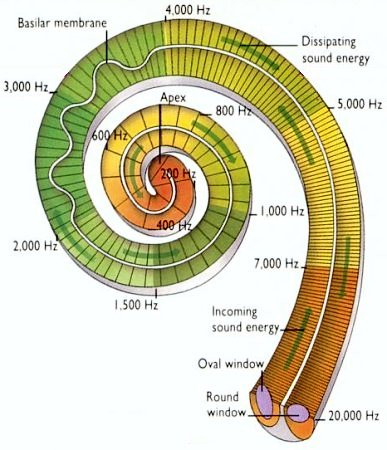
\includegraphics[width=0.6\textwidth]{cochlea}
    \caption{Cochlea divided by frequency regions \cite{scienceblogs.2010.05.10}.}
    \label{fig:cochlea}
\end{figure}

A key factor in the perception of speech and other sounds is \emph{loudness}, a
quality related to the physical property of sound pressure level. Loudness is
quantified by relating the actual sound pressure level of a pure tone (in dB
relative to a standard reference level) to the perceived loudness of the same
tone (in a unit called phons) over the range of human hearing (20 Hz–20 kHz)
\cite{rabiner.schafer.2007}. As shown in \figureref{loudness}, a 100 Hz tone
at 60 dB is equal in loudness to a 1000 Hz tone at 50 dB, both having the
\emph{loudness level} of 50 phons (by convention).


\begin{figure}[ht]
    \centering
    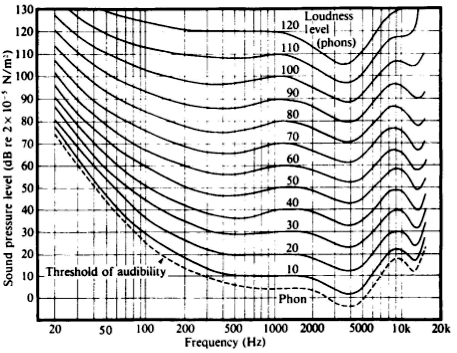
\includegraphics[width=\textwidth]{loudness}
    \caption{Loudness level for human hearing \cite{fletcher.munson.1933}.}
    \label{fig:loudness}
\end{figure}


\subsection{The Mel Scale}

The mel scale is the result of an experiment conducted by Stevens, Volkmann and
Newman \cite{stevens.volkmann.newman.1937} intended to measure the perception
of a pitch and construct a scale based on it. Each observer was asked to listen
to two tones, one in the fixed frequencies 125, 200, 300, 400, 700, 1000, 2000,
5000, 8000 and 12000 Hz, and the other free to have its frequency varied by the
observer for each fixed frequency of the first tone. An interval of 2 seconds
separated both tones. The observers were instructed to say in which frequency the
second tone was ``half the loudness" of the first. A geometric mean was taken from
the observers' answers and a measure of 1000 mels was assigned to the frequency
of 1000 Hz, 500 mels to the frequency sounding half as high (as determined by Fig. 1
in \cite{stevens.volkmann.newman.1937}) and so on.

Decades after the creation of the mel scale, O'Shaughnessy \cite{oshaughnessy.1987}
published an equation to convert frequencies in hertz to frequencies in mels.

\begin{equation}
    f_{mel} = 2595 log_{10}(1 + \frac{f}{700})
    \label{eq:mel_conversion}
\end{equation}
\\
\noindent Being logarithmic, the growth of a mel-frequency curve is slow with a
linear growth of the frequency in hertz. \equationref{mel_conversion} sometimes
is used only for frequencies higher than 1000 Hz while the lower frequencies obey
a linear function. In this work all conversions will use \equationref{mel_conversion},
as shown by \figureref{mel_scale}.

\begin{figure}[ht]
    \centering
    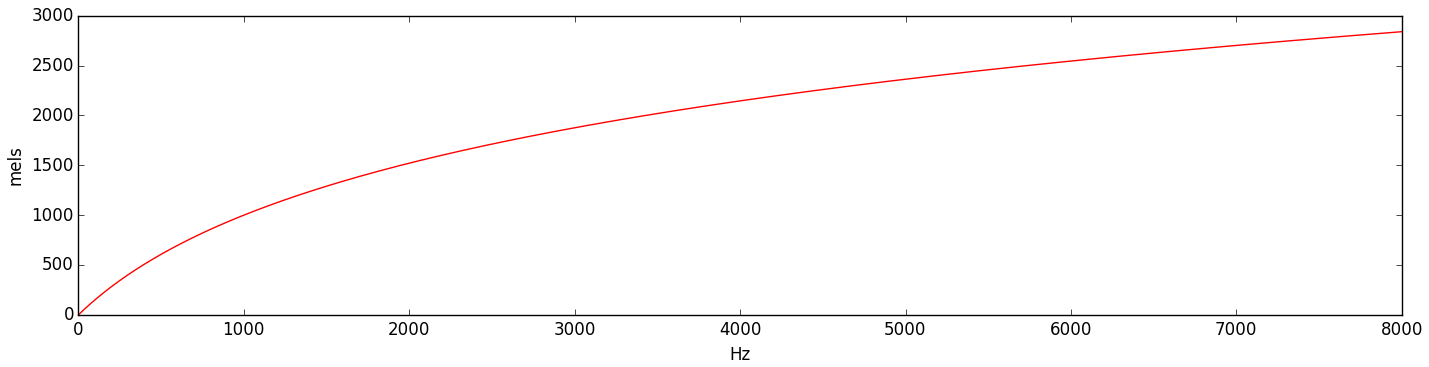
\includegraphics[width=\textwidth]{mel_scale}
    \caption{The logarithm curve of the mel-frequency.}
    \label{fig:mel_scale}
\end{figure}


\subsection{Cepstrum}


\subsection{Extraction Process}


\subsubsection{Pre-emphasis}